
\BiChapter{相关理论}{TODO}
\label{chap:part2}

\BiSection{光场技术基本理论}{TODO}

光场的概念最早由A.Gershun~\cite{gershun1939light}教授提出,是空间中光线集合的完备表示,采集并显示光场就能在视觉上重现真实世界。
1991年,MIT的Edward H.Adelson教授和James R.Bergen\cite{adelson1991plenoptic}教授指出人眼对光线的视觉感知可以认为是沿着单一函数的一个或多个方向的局部变化,描述了光照射到观察面的信息结构。
一旦定义了这个函数,各种潜在的视觉属性(如运动、颜色和方向)的测量就能够自动分离出来。
这个函数被称为全光函数,表示为:
%$$$$
\begin{equation}
	P(x,y,z,\theta,\varphi,\lambda,t)
\end{equation}\par
其中$(x,y,z)$为发光物体的空间位置,$(\theta,\varphi)$分别表示传播光线入射的垂直角度和水平角度,$\lambda$表示传播光线的波长,发光物体所发射的光线信息随时时间$t$的推移而变化。
然而,这种能够记录空间中光线信息的七维全光函数过于复杂、数据量大,难以记录和存储,在实际计算中并未得到应用。
需要对其进行简化处理。
McMillan等~\cite{mcmillan2023plenoptic}在七维全光函数的基础上提出了
简化波长$\lambda$和时间$t$的更为方便的五维光场模型。
\begin{equation}
	P(x,y,z,\theta,\varphi)
\end{equation}\par
五维光场模型通过记录红、绿、蓝三原色来简化波长$\lambda$,以及通过记录不同帧来简化时间$t$。
实际上,光线在空间传播中,因传播距离而造成的信息损耗微乎其微,光场模型还可以进一步简化。
%如果不考虑光线在空间传播过程中的衰减,记录光场信息的五维模型还可以进一步简化成四参数光场函数。
%\par
\begin{figure}[!ht]
	\centering
	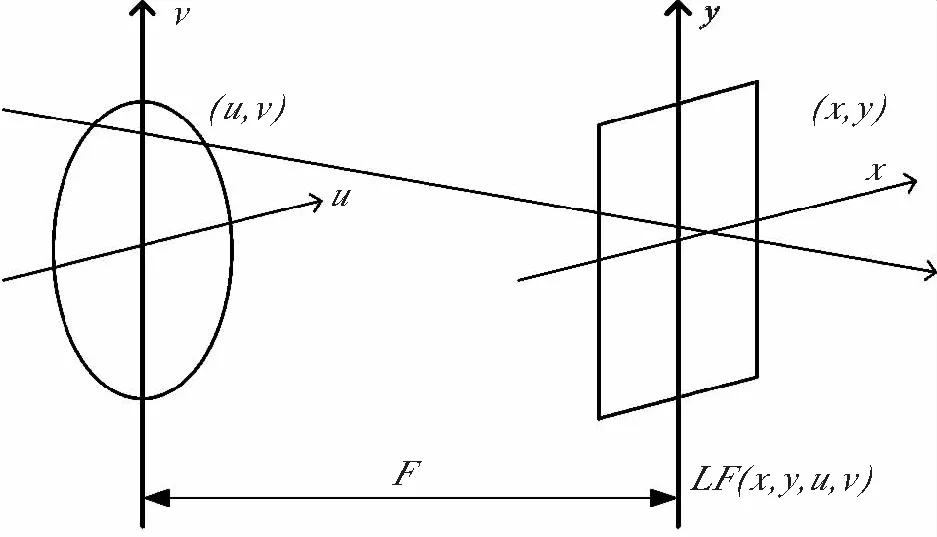
\includegraphics[width=0.70\linewidth]{figures/chapter2/double-plane2}
	\bicaption{光场双平面四参数模型}{Light field biplane four-parameter model}  
	\label{chapter2_fig1:double_plane}
\end{figure}
Levoy等~\cite{levoy2023light}忽略掉传播距离维度$z$得到四维光场模型,
同时提出光场渲染理论和双平面模型来描述静态的可见光。
双平面模型利用两个互相平行的参数化平面表示四维光场。
假设光线在没有遮挡物和散射介质的区域,忽略光线在传播过程中波长和时间维度的变化,
则任意一个包含位置和方向信息的光线都可以用双平面参数来表示,
空间中的光线穿过这两个平面分别相交于点$(u, v)$和点$(s, t)$,
光线即可用四维光场函数表示,如图~\ref{chapter2_fig1:double_plane}~所示,其模型参数如下:
\begin{equation}
	P(u, v, x, y)
\end{equation}\par
在光场成像设备中,我们可以用$(u, v)$表示光线与微透镜阵列的交点,用$(s, t)$表示光线与CCD传感器探测面的交点。一条光线在整个四维空间中对应着光场的一个采样点。四维光场理论的推出为全光相机、相机阵列等设备提供了理论基础。目前,大多数单体全光相机和相机阵列的光场采集设备都遵循着四维光场理论。
%
%
%发展出了适用于光学系统的光场双平面参数特征。
%假设一条光线在两个不共面的平面$(u,v)$和平面$(s,t)$各有一个交点,则该光线可以用这两个交点唯一表示。
% \emph{et~al.}~
%光场是计算机科学领域的学者定义的“Light Field”,是指除了包含原图像矩阵中的空间坐标$(x,y)$和强度$I$外,还有光线入射的角度信息$(\theta,\varphi)$。
%光在传播过程中的各种潜在的视觉属性(如运动、颜色和方向)。


\BiSubsection{光场成像原理}{TODO}
在传统成像中,光线被捕获并呈现到成像平面上。然而,光场成像采用不同的方式。
它是一种计算成像技术,旨在捕获光线强度的同时记录光线的传播方向。
为了得到可视化的图像信息,必须对捕获的光场信息进行计算处理。
根据成像设备或记录方法的不同,现有的光场成像方式可以分为多传感器采集成像、
时间序列采集成像、空域复用成像和频域复用成像。\par
\begin{figure}[!ht]
	\centering
	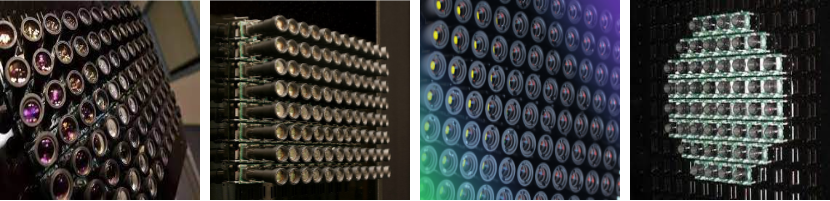
\includegraphics[width=1\linewidth]{figures/chapter2/camera_array}
	\bicaption{相机阵列光场成像}{Camera array for light field imaging}  
	\label{chapter2_fig2:camera_array}
\end{figure}
(1)使用相机阵列获取光场信息是通过多个相机以特定的空间分布在不同视角下捕获场景图像的方法,
如图~\ref{chapter2_fig2:camera_array}~所示。
每个相机捕获的是四维光场在其相对于场景方向上的二维投影。
通过融合这些相机捕获的图像,就可以获得完整的四维光场数据。
大尺度空间相机阵列主要应用于合成孔径成像以实现“透视”监测,或通过拼接实现大视角全景成像。
相比之下,紧密排列的相机阵列则主要用于捕获高性能动态场景或场景的三维分布和结构等信息。
光场数据的空间解析度取决于传感器本身,而角度解析度由传感器数量和布局方式确定。
这种采集方法能够在单次曝光中瞬时捕捉光场,因此还能记录光场的时间序列信息。
尽管这种成像方法空间解析度较高,但却带来了庞大的图像数据量,因此处理上更加耗时。
此外,这种成像方式对多传感器的相对位置要求也较高。\par
%
%
%
%
\begin{figure}[!ht]
	\centering
	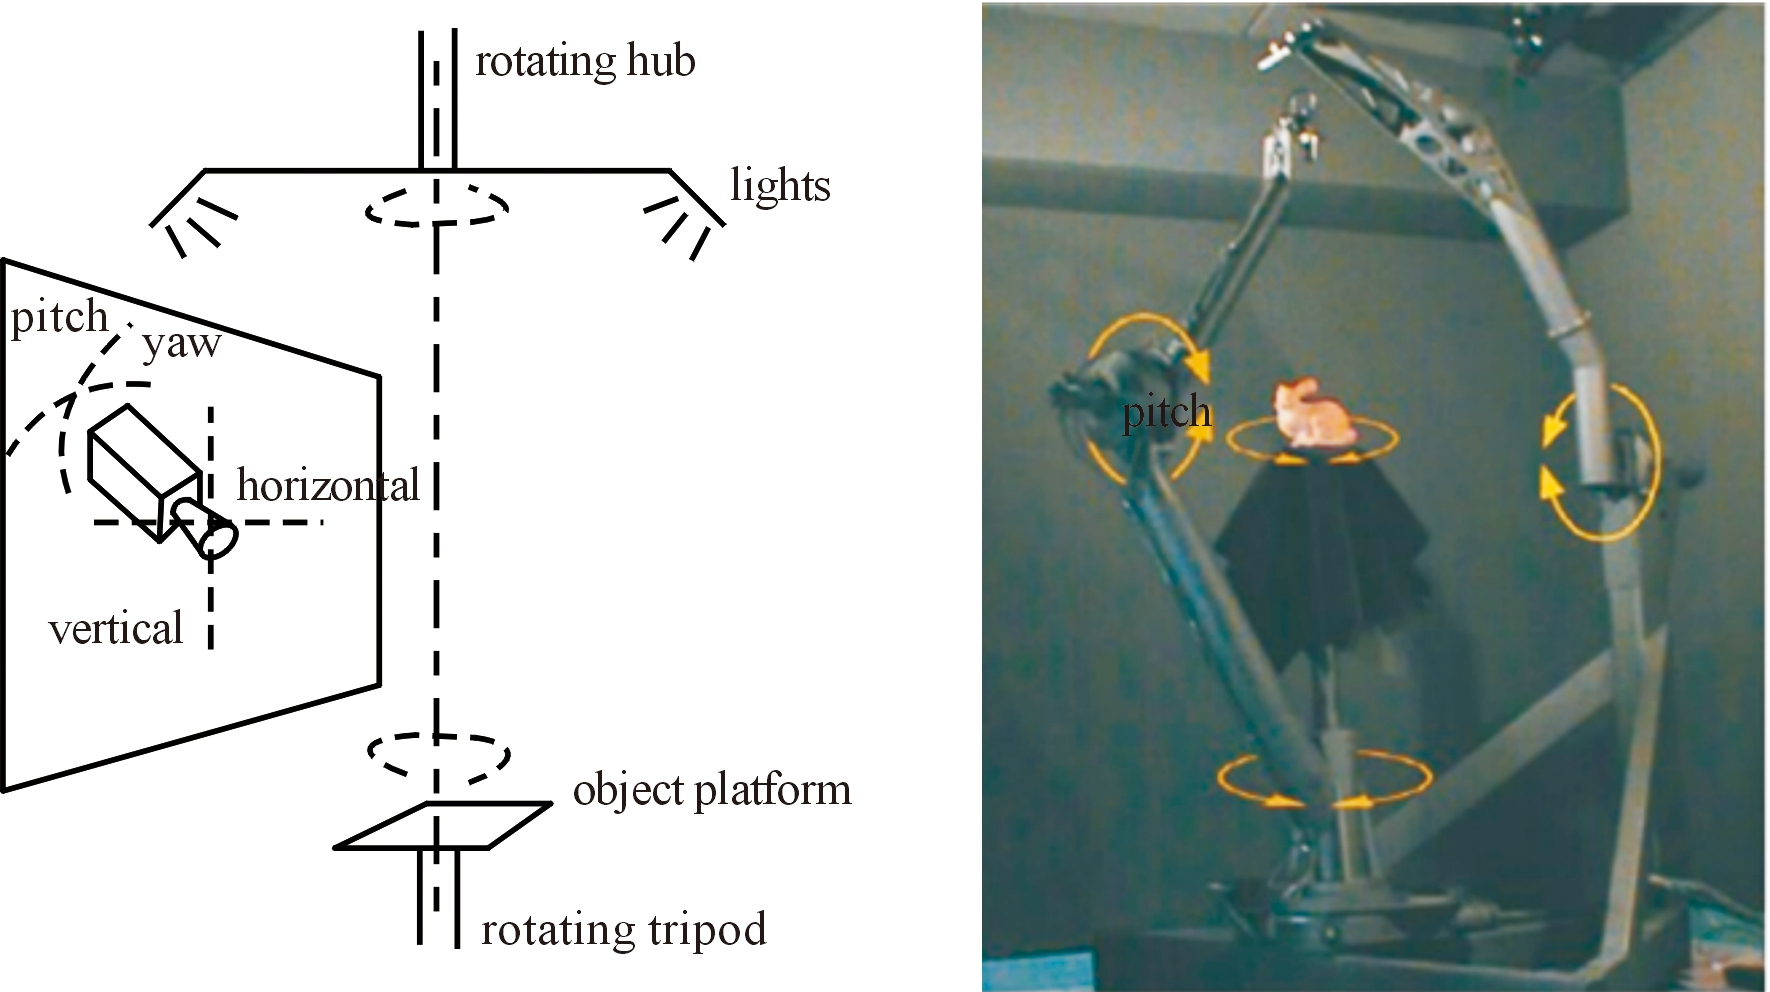
\includegraphics[width=0.7\linewidth]{figures/chapter2/time_seq2}
	\bicaption{时间序列光场成像}{TODO}  
	\label{chapter2_fig3:time_seq2}
\end{figure}
(2)除了多个相机阵列排布外,Marc Levoy等人\cite{levoy2023light}采用了单相机扫描系统。
他们通过让相机在固定的导轨上移动,分时获取不同空间视角下的场景图像,
最后将这些图像进行融合,从而实现相同的功能。
图~\ref{chapter2_fig3:time_seq2}~是典型的时序采集光场信息的示例。
与多传感器采集相比,这种方法的优势在于能够实现高密度角度分辨率的光场信息采集。
然而,缺点也显而易见,即需要高精度的控制,并且相对于多传感器采集,这种成像方式也更加耗时。
这些缺点限制了该成像方式仅适用于静态场景的光场信息采集。\par
%
%
%然而,由于需要进行扫描,这种方法更适用于静态场景的光场测量。
%此外,测量的精度受到相机移动定位精度的影响。
% 图3和图4展示了相机阵列以及单相机路径扫描方案实现光场信息获取的示例。
%
%
%
\begin{figure}[!ht]
	\centering
	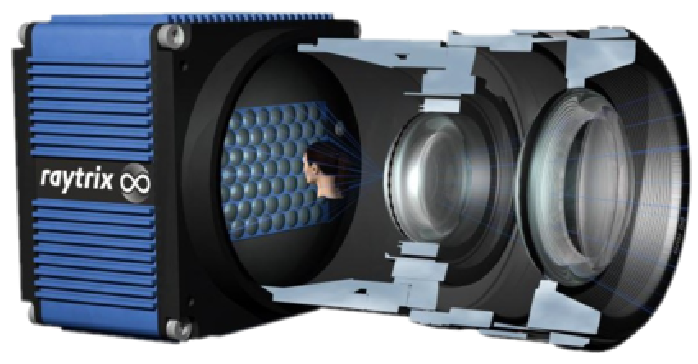
\includegraphics[width=0.90\linewidth]{figures/chapter2/microlens_for_lf_imaging2.drawio}
	\bicaption{微透镜光场成像}{TODO}  
	\label{chapter2_fig4:microlens_for_lf_imaging}
\end{figure}
(3)空域复用的成像方式通过在图像传感器上安装微透镜阵列来实现,这是光场采集中常见的方式之一。
图~\ref{chapter2_fig4:microlens_for_lf_imaging}~展示了这种空域复用的成像方式的工作原理:通过将微透镜阵列插入普通成像系统的主透镜的一次像面,每个微透镜单元及其对应的传感器区域记录了光线从不同视角成像的集合,从而获得包含位置和传播方向的四维光场数据。
空域复用的成像方式优势在于结构紧凑,一次曝光即可捕捉光线强度与方向,适用于不同场景和动态场景的光场信息采集。
1992年,Adelson~\cite{adelson1992single}及其团队首次提出了利用微透镜阵列的光场相机模型;
然而,这种空域复用方式需要在空间分辨率和角度分辨率之间进行权衡。
当角度分辨率最大时,微透镜与图像传感器重合,空间分辨率最小;反之亦然。
为解决这一问题,
Georgiev~\cite{georgiev2010focused}在2021年提出了可调整微透镜与图像传感器相对位置的聚焦光场相机结构,
实现了角度分辨率与空间分辨率的动态调整。
%
% 相机阵列的体积庞大,限制了其应用范围。
% 通过缩小相机阵列中各成像单元之间的基线,可以在单个相机框架下利用微透镜阵列来采集光场信息。
% 空域复用的成像方式通过在图像传感器上安装微透镜阵列来实现,这是光场采集中常见的方式之一,可通过单次曝光捕获光场信息。
%
%
\BiSubsection{光场数据可视化}{TODO}






\BiSection{光场显著性目标检测相关理论}{TODO}

\BiSubsection{基于多视角图像的显著性目标检测原理}{TODO}
\BiSubsection{基于焦点堆栈的显著性目标检测原理}{TODO}
\BiSubsection{显著性目标检测性能评估指标}{TODO}


\BiSection{本章小节}{TODO}

本章首先阐述了光场技术的基本理论,介绍了光场的成像原理以及数据可视化形式;
然后介绍了光场显著性目标检测的相关理论,分别描述了基于多视角图像的显著性目标检测、
基于焦点堆栈的显著性目标检测方法的实现原理,
并引入了显著性目标检测中常用的几种性能评价指标。